\documentclass[a4paper, 11pt]{article}
\usepackage[utf8]{inputenc}
\usepackage[left=18mm, right=18mm, top=22mm, bottom=22mm]{geometry}

\usepackage{amsmath,amsfonts,amssymb,bm}
\usepackage[english]{babel}
\usepackage{hyperref}
\usepackage{xcolor}
\usepackage{fancyhdr}
\usepackage{graphicx}
\usepackage{booktabs}
\usepackage{float}
\usepackage{listings}
\usepackage{tikz}
\usetikzlibrary{shapes.geometric, arrows, positioning, fit, backgrounds}

% Style settings
\definecolor{harvardcrimson}{HTML}{8C1D40}
\definecolor{softgrey}{HTML}{F3F3F3}
\definecolor{kwcol}{HTML}{1F4E79}
\definecolor{codebg}{HTML}{F5F5F5}
\definecolor{codegreen}{HTML}{228B22}
\definecolor{codepurple}{HTML}{9932CC}

\hypersetup{
  colorlinks=true,
  linkcolor=harvardcrimson,
  citecolor=harvardcrimson,
  urlcolor=harvardcrimson,
}

\pagestyle{fancy}
\fancyhf{}
\rhead{\textcolor{harvardcrimson}{\textbf{GPU Pipeline Review}}}
\lhead{\textcolor{harvardcrimson}{\textbf{y3\_cluster\_cpp}}}
\cfoot{\thepage}
\renewcommand{\headrulewidth}{0.4pt}
\renewcommand{\footrulewidth}{0.4pt}
\setlength{\headheight}{14pt}
\renewcommand{\baselinestretch}{1.12}

% Code listing style
\lstset{
  backgroundcolor=\color{codebg},
  basicstyle=\ttfamily\small,
  breaklines=true,
  commentstyle=\color{codegreen},
  keywordstyle=\color{kwcol}\bfseries,
  stringstyle=\color{codepurple},
  frame=single,
  framesep=5pt,
  rulecolor=\color{gray},
  showstringspaces=false,
  tabsize=2,
  language=C++,
  morekeywords={__device__, __host__, double, void, class, struct, explicit, const}
}

\newcommand{\modname}[1]{\textcolor{kwcol}{\texttt{#1}}}
\newcommand{\filepath}[1]{{\small\texttt{#1}}}

\title{\vspace{-4ex}\huge \textbf{GPU Pipeline Review \& Architecture Recommendations}\\[0.5ex]
       \Large \textbf{simple\_gpu module analysis and roadmap}}
\author{Claude Code Review}
\date{2026-05-25 (Updated: Testing Progress)}

\begin{document}
\maketitle

\tableofcontents
\vspace{1em}

% ============================================================================
\section{Testing Progress \& Status}
\label{sec:status}

\subsection{Decision: Direct Integration Approach (Option B)}

After review, the team decided to pursue \textbf{Option B: Direct 4D Integration} rather than porting the selection function. The rationale:

\begin{itemize}
  \setlength\itemsep{2pt}
  \item \textbf{Independent Validation}: GPU code can be tested independently of the CPU \texttt{sel\_function} pipeline
  \item \textbf{Cross-Validation}: If both approaches yield the same results, both implementations are validated
  \item \textbf{Simpler Dependencies}: No need to match the exact $S_{ij}$ tabulation grid
\end{itemize}

\subsection{Modules Implemented}

\begin{table}[H]
\centering
\small
\begin{tabular}{@{}l l l@{}}
\toprule
Module & Status & Notes \\
\midrule
\texttt{numberCountsSimple} & \textcolor{green!50!black}{\textbf{TESTED}} & 3D integration $(l_o, z_t, \ln M)$ \\
\texttt{sigma1hSimple} & Built & Awaiting haloModel \\
\texttt{sigmaTotSimple} & Built & Awaiting haloModel \\
\texttt{shearTotSimple} & Built & Awaiting haloModel \\
\texttt{numberCountsFull} & Built & 4D integration with EMG \\
\bottomrule
\end{tabular}
\caption{GPU module implementation status.}
\end{table}

\subsection{Test Results: \texttt{numberCountsSimple}}

Successfully tested on HPC (2026-05-25). Integration over $(l_o, z_t, \ln M)$ with MOR and photo-z kernel.

\begin{table}[H]
\centering
\begin{tabular}{@{}c c c c c@{}}
\toprule
Bin & $z$ Range & $N$ (counts) & Error & Rel.\ Error \\
\midrule
1 & $[0.20, 0.35]$ & 4825.6 & $\pm$4.15 & 0.09\% \\
2 & $[0.35, 0.50]$ & 7716.8 & $\pm$6.97 & 0.09\% \\
3 & $[0.50, 0.65]$ & 7984.7 & $\pm$4.81 & 0.06\% \\
\bottomrule
\end{tabular}
\caption{GPU number counts results for 3 redshift bins ($\lambda_{\rm ob} \in [10, 200]$).}
\end{table}

\paragraph{Integration Parameters:}
\begin{lstlisting}[language=bash]
lo_low = 10.0, lo_high = 200.0
zt_low = 0.1, zt_high = 0.8
lnm_low = 31.0, lnm_high = 36.0
eps_rel = 1e-3, algorithm = pagani
\end{lstlisting}

\paragraph{Timing:} Module execution took 0.05 seconds (after 0.5s setup).

\subsection{New CUDA Models Created}

\paragraph{\texttt{emg\_des\_t.cuh}} -- EMG kernel $P(\lambda_{\rm ob}|\lambda_{\rm tr},z)$
\begin{itemize}
  \item Implements Costanzi observation scatter model
  \item Uses \texttt{erfcx} for numerical stability at large arguments
  \item Spline-interpolated parameters: $\mu(z), \sigma(z), \tau(z), f_{\rm prj}(z)$
\end{itemize}

\paragraph{\texttt{numberCountsFull.cu}} -- Full 4D integration
\begin{itemize}
  \item Integrates over $(\lambda_{\rm ob}, \lambda_{\rm tr}, z_t, \ln M)$
  \item Includes EMG scatter via \texttt{emg\_des\_t.cuh}
  \item Grid points: richness bins $\times$ redshift bins
\end{itemize}

\subsection{Files Added to Repository}

\begin{itemize}
  \setlength\itemsep{2pt}
  \item \filepath{src/models/emg\_des\_t.cuh} -- EMG CUDA model
  \item \filepath{src/modules/simple\_gpu/numberCountsFull.cu} -- 4D integration
  \item \filepath{src/modules/simple\_gpu/plob\_ltr\_loader.py} -- EMG coefficient loader
  \item \filepath{cosmosis\_tests/gpu/number\_counts\_simple\_test.ini} -- Minimal test config
  \item \filepath{cosmosis\_tests/gpu/number\_counts\_full\_test.ini} -- 4D test config
  \item \filepath{cosmosis\_tests/gpu/values\_simple\_gpu.ini} -- Parameter values
\end{itemize}

Branch: \texttt{gpu-pipeline} on \texttt{marcpaterno/y3\_cluster\_cpp}

% ============================================================================
\section{Code Review: What You've Built}
\label{sec:review}

\subsection{Strengths}

\paragraph{1. Clean Module Pattern.}
Your modules follow the established \texttt{CosmoSISSICUDAModule<T>} template pattern well:

\begin{lstlisting}
set_sample(DataBlock&)    // Construct CUDA models from datablock
set_grid_point(pt)        // Set current bin parameters
operator()(lo, zt, lnM)   // The integrand, __host__ __device__
\end{lstlisting}

\paragraph{2. Proper CUDA Model Usage.}
You're correctly using existing \texttt{\_\_device\_\_ \_\_host\_\_} models:
\begin{itemize}
  \setlength\itemsep{2pt}
  \item \texttt{HMF\_t} -- handles mass-axis shift internally
  \item \texttt{MOR\_DES\_LOG\_t} -- correct Costanzi-2019 skew-normal MOR
  \item \texttt{DV\_DO\_DZ\_t}, \texttt{OMEGA\_Z\_DES} -- cosmology pieces
\end{itemize}

\paragraph{3. Memory Footprint Tracking.}
Good that you include \texttt{get\_device\_mem\_footprint()}.

\paragraph{4. Integration Infrastructure.}
PAGANI GPU integrator is already wired in via \texttt{CosmoSISSICUDAModule}.

\subsection{Issues Found}

\paragraph{Issue 1: \texttt{sig\_max.cuh} uses \texttt{std::max} instead of sum.}

\begin{lstlisting}[title={\filepath{src/models/sig\_max.cuh:67}}]
double const res = std::max(sig_1, sig_2);  // Should be sig_1 + sig_2
\end{lstlisting}

This returns $\max(\Sigma_{1h}, b \cdot \Sigma_{2h})$ instead of $\Sigma_{1h} + b \cdot \Sigma_{2h}$. The total surface density should be the sum.

\paragraph{Issue 2: Missing richness binning.}
Your integrand integrates over all $\lambda_{\rm ob} \in [10, 200]$:

\begin{lstlisting}[language=bash]
lo_low = 10.0
lo_high = 200.0
\end{lstlisting}

But DES Y3 uses discrete bins $[20,30], [30,45], [45,60], [60,200]$. You're computing a single count over all richness.

\paragraph{Issue 3: Photo-z kernel vs richness selection.}
You're using \texttt{INT\_ZO\_ZT\_DES\_t} which is a Gaussian photo-z smearing kernel $K(z_{\rm ob}|z)$:

\begin{lstlisting}
double const photoz = (*int_zo_zt_)(zo_low_, zo_high_, zt);
\end{lstlisting}

This is correct for z-binning, but the production pipeline also includes:
\begin{itemize}
  \setlength\itemsep{2pt}
  \item EMG convolution $P(\lambda_{\rm ob}|\lambda_{\rm tr},z)$
  \item Richness kernel $K_i(\lambda_{\rm tr},z)$ as CDF difference
\end{itemize}

\paragraph{Issue 4: \texttt{sigma1hSimple} missing from ini.}
The \filepath{simple\_gpu\_test.ini} only runs \texttt{numberCountsSimple}, \texttt{sigmaTotSimple}, \texttt{shearTotSimple} -- missing \texttt{sigma1hSimple}.

% ============================================================================
\section{Architecture: Path to Full GPU Pipeline}
\label{sec:architecture}

\subsection{Option A: Port Selection Function to GPU (Recommended)}

This matches the CPU approach: pre-compute $S_{ij}$ on GPU, then do 2D integrals.

\begin{figure}[H]
\centering
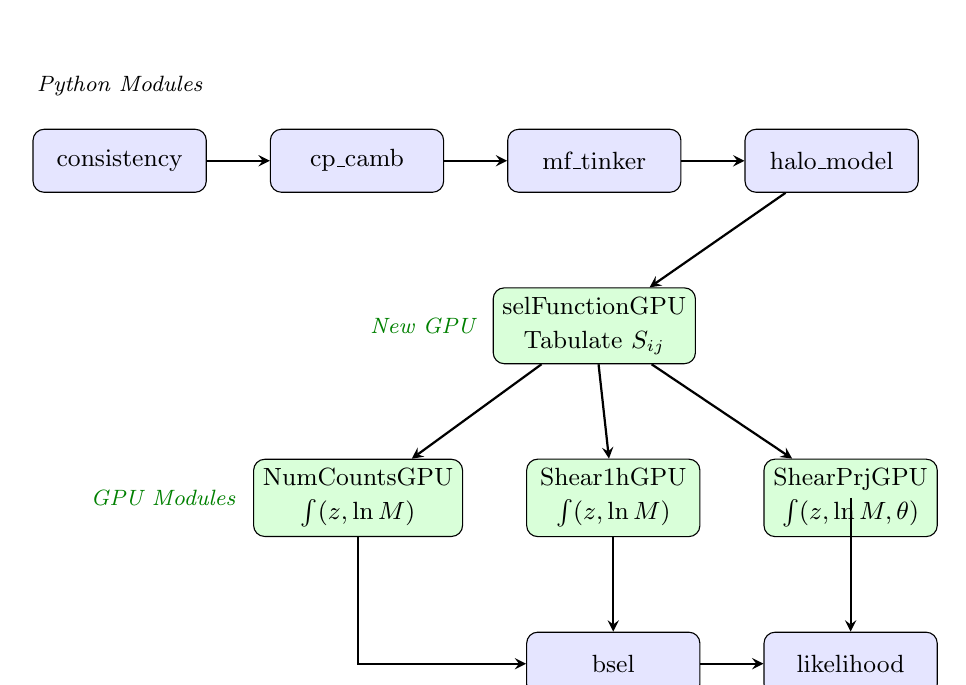
\begin{tikzpicture}[
  node distance=0.8cm,
  box/.style={rectangle, draw, rounded corners, minimum width=2.2cm, minimum height=0.8cm, align=center, font=\small},
  pybox/.style={box, fill=blue!10},
  gpubox/.style={box, fill=green!15},
  arrow/.style={->, thick, >=stealth}
]

% Python modules row 1
\node[pybox] (consistency) {consistency};
\node[pybox, right=of consistency] (cpcamb) {cp\_camb};
\node[pybox, right=of cpcamb] (mftinker) {mf\_tinker};
\node[pybox, right=of mftinker] (halomodel) {halo\_model};

\draw[arrow] (consistency) -- (cpcamb);
\draw[arrow] (cpcamb) -- (mftinker);
\draw[arrow] (mftinker) -- (halomodel);

% GPU selection function
\node[gpubox, below=1.2cm of mftinker] (selfunc) {selFunctionGPU\\Tabulate $S_{ij}$};
\draw[arrow] (halomodel) -- (selfunc);

% GPU integration modules
\node[gpubox, below=1.2cm of selfunc, xshift=-3cm] (numcounts) {NumCountsGPU\\$\int(z,\ln M)$};
\node[gpubox, right=of numcounts] (shear1h) {Shear1hGPU\\$\int(z,\ln M)$};
\node[gpubox, right=of shear1h] (shearprj) {ShearPrjGPU\\$\int(z,\ln M,\theta)$};

\draw[arrow] (selfunc) -- (numcounts);
\draw[arrow] (selfunc) -- (shear1h);
\draw[arrow] (selfunc) -- (shearprj);

% Python modules row 2
\node[pybox, below=1.2cm of shear1h] (bsel) {bsel};
\node[pybox, right=of bsel] (likelihood) {likelihood};

\draw[arrow] (numcounts) |- (bsel);
\draw[arrow] (shear1h) -- (bsel);
\draw[arrow] (shearprj) -| (likelihood);
\draw[arrow] (bsel) -- (likelihood);

% Labels
\node[above=0.3cm of consistency, font=\footnotesize\itshape] {Python Modules};
\node[left=0.1cm of selfunc, font=\footnotesize\itshape, text=green!50!black] {New GPU};
\node[left=0.1cm of numcounts, font=\footnotesize\itshape, text=green!50!black] {GPU Modules};

\end{tikzpicture}
\caption{Recommended GPU pipeline architecture with pre-tabulated $S_{ij}$.}
\label{fig:architecture}
\end{figure}

\paragraph{Pros:}
\begin{itemize}
  \setlength\itemsep{2pt}
  \item Matches CPU pipeline semantics exactly
  \item $S_{ij}$ tabulation is embarrassingly parallel (one thread per $(\ln M, z, \text{bin})$ point)
  \item Downstream integrals stay 2D (fast)
  \item Easy validation against CPU
\end{itemize}

\paragraph{Cons:}
\begin{itemize}
  \setlength\itemsep{2pt}
  \item Need to port EMG/erfcx to CUDA (but CUDA has \texttt{erfcf}/\texttt{erfc})
  \item Extra memory for $S_{ij}$ tables on device
\end{itemize}

\subsection{Option B: Direct 3D Integration (Your Current Approach)}

Keep integrating over $(\lambda_{\rm ob}, z_t, \ln M)$ directly.

\paragraph{To make this work for production:}

\begin{enumerate}
  \item \textbf{Add richness bins} -- Split $\lambda_{\rm ob}$ integration by bin:
\begin{lstlisting}[language=bash]
lo_low = 20.0   // bin 0
lo_high = 30.0
// ... etc for each bin
\end{lstlisting}

  \item \textbf{Add EMG kernel} -- Create \texttt{EMG\_KERNEL\_t} CUDA model:
\begin{lstlisting}
// P(lambda_ob | lambda_tr, z) EMG distribution
__device__ __host__ double
operator()(double lob, double ltr, double z) const {
  // EMG CDF difference for bin edges
}
\end{lstlisting}

  \item \textbf{Increase dimensionality} -- Integrate over $(\lambda_{\rm ob}, \lambda_{\rm tr}, z_t, \ln M) = 4$D
\end{enumerate}

\paragraph{Pros:}
\begin{itemize}
  \setlength\itemsep{2pt}
  \item No pre-tabulation step
  \item Potentially more accurate (no interpolation of $S_{ij}$)
\end{itemize}

\paragraph{Cons:}
\begin{itemize}
  \setlength\itemsep{2pt}
  \item 4D integration is much slower than 2D
  \item PAGANI may struggle with high-dimensional integrals
  \item Harder to validate
\end{itemize}

% ============================================================================
\section{Updated Implementation Roadmap (Option B)}
\label{sec:roadmap}

\textbf{Note:} The roadmap has been updated to reflect the decision to use direct integration (Option B) rather than porting the selection function.

\subsection{Phase 1: Validate Simple Modules (1--2 days)}

\begin{itemize}
  \item[\textcolor{green!50!black}{$\checkmark$}] Test \texttt{numberCountsSimple} -- \textbf{DONE}
  \item[$\square$] Fix \texttt{sig\_max.cuh} to use sum instead of max
  \item[$\square$] Create haloModel or equivalent to provide GPU tables
  \item[$\square$] Test \texttt{sigma1hSimple}, \texttt{sigmaTotSimple}, \texttt{shearTotSimple}
\end{itemize}

\subsection{Phase 2: Test Full 4D Integration (1--2 days)}

\begin{itemize}
  \item[\textcolor{green!50!black}{$\checkmark$}] Create \texttt{emg\_des\_t.cuh} -- \textbf{DONE}
  \item[\textcolor{green!50!black}{$\checkmark$}] Create \texttt{numberCountsFull.cu} -- \textbf{DONE}
  \item[$\square$] Test \texttt{numberCountsFull} with DES Y3 bins:
\begin{lstlisting}[language=bash]
# Richness bins: [20,30], [30,45], [45,60], [60,200]
# Redshift bins: [0.20,0.35], [0.35,0.50], [0.50,0.65]
\end{lstlisting}
  \item[$\square$] Verify EMG parameters load correctly from \texttt{plob\_ltr\_params.npz}
  \item[$\square$] Check 4D integration convergence (may need higher \texttt{max\_eval})
\end{itemize}

\subsection{Phase 3: Create GPU haloModel (2--3 days)}

The sigma/shear modules require tables from haloModel:
\begin{itemize}
  \item[$\square$] $\Sigma_{\rm nfw}(R, \ln M, z)$ -- NFW surface density
  \item[$\square$] $\Sigma_{\rm hh}(R, z)$ -- 2-halo term (halo-halo)
  \item[$\square$] $\Delta\Sigma_{\rm nfw}(R, \ln M, z)$ -- NFW excess surface density
  \item[$\square$] $b(\ln M, z)$ -- halo bias
  \item[$\square$] $\Sigma_{\rm crit}^{-1}(z)$ -- critical surface density inverse
\end{itemize}

Options:
\begin{enumerate}
  \item Port \filepath{y3\_buzzard/haloModel.py} to CosmoSIS module format
  \item Create GPU-native haloModel using existing CUDA interpolators
\end{enumerate}

\subsection{Phase 4: GPU Shear/Sigma Validation (2--3 days)}

\begin{itemize}
  \item[$\square$] Test \texttt{sigmaTotSimple} output: $N \times \langle\Sigma_{\rm tot}(R)\rangle$
  \item[$\square$] Test \texttt{shearTotSimple} output: $N \times \langle\gamma_t(R)\rangle$
  \item[$\square$] Divide by \texttt{numberCountsSimple} to get bin-averaged profiles
  \item[$\square$] Compare against CPU pipeline with equivalent physics
\end{itemize}

\subsection{Phase 5: Cross-Validation (2--3 days)}

\begin{itemize}
  \item[$\square$] Run CPU pipeline with \texttt{sel\_function} on same cosmology
  \item[$\square$] Compare number counts: GPU direct vs CPU $S_{ij}$ approach
  \item[$\square$] If results match to $<1\%$, both implementations are validated
  \item[$\square$] Document any systematic differences
\end{itemize}

% ============================================================================
\section{Key Technical Recommendations}
\label{sec:technical}

\subsection{Memory Management}

\begin{lstlisting}
// Pre-allocate device memory once in setup(), reuse across samples
class ModuleGPU {
  thrust::device_vector<double> d_S_ij_;  // Persists across samples

  void set_sample(DataBlock& sample) {
    // Only update values, don't reallocate
    thrust::copy(h_S_ij.begin(), h_S_ij.end(), d_S_ij_.begin());
  }
};
\end{lstlisting}

\subsection{Interpolation Tables}

The existing \texttt{quad::Interp2D} handles device memory internally. Use it for all lookup tables (HMF, bias, $\Sigma_{\rm nfw}$, etc.).

\subsection{Integration Strategy}

For the projection integrand (\texttt{red\_shear\_prj}), consider:
\begin{itemize}
  \setlength\itemsep{2pt}
  \item \textbf{Fixed GL panels} (current CPU approach) -- easy to parallelize per wall point
  \item \textbf{Batch integration} -- integrate all $(\lambda_{\rm ob}, z_{\rm ob}, R)$ points simultaneously
\end{itemize}

\subsection{MPI + GPU}

Your \texttt{DeviceInitializer} already handles MPI rank $\to$ GPU mapping. For multi-node runs:

\begin{lstlisting}
// Each MPI rank gets one GPU
DeviceInitializer(mpi_info const& info) : id(info.local_rank)
\end{lstlisting}

% ============================================================================
\section{Quick Wins \& Immediate Next Steps}
\label{sec:quickwins}

\subsection{Completed}

\begin{itemize}
  \item[\textcolor{green!50!black}{$\checkmark$}] \texttt{numberCountsSimple} validated with sub-0.1\% integration error
  \item[\textcolor{green!50!black}{$\checkmark$}] EMG model implemented (\texttt{emg\_des\_t.cuh})
  \item[\textcolor{green!50!black}{$\checkmark$}] 4D module built (\texttt{numberCountsFull.cu})
  \item[\textcolor{green!50!black}{$\checkmark$}] Test configurations in \filepath{cosmosis\_tests/gpu/}
\end{itemize}

\subsection{Immediate Next Steps}

\paragraph{1. Test \texttt{numberCountsFull}:}
\begin{lstlisting}[language=bash]
cosmosis ${Y3_CLUSTER_CPP_DIR}/cosmosis_tests/gpu/number_counts_full_test.ini
\end{lstlisting}

This tests the full physics with EMG observation scatter $P(\lambda_{\rm ob}|\lambda_{\rm tr},z)$.

\paragraph{2. Fix the \texttt{std::max} bug} in \texttt{sig\_max.cuh} before any shear comparisons.

\paragraph{3. Create/adapt haloModel} to provide NFW and 2-halo tables for sigma/shear modules.

\paragraph{4. Validation comparison:}
\begin{lstlisting}[language=Python]
# Compare GPU numberCountsFull vs CPU NumCountsSel
# Both should give same N_i for identical cosmology + MOR parameters
\end{lstlisting}

% ============================================================================
\section{Summary}
\label{sec:summary}

\begin{table}[H]
\centering
\small
\begin{tabular}{@{}l l l l@{}}
\toprule
Phase & Effort & Priority & Status \\
\midrule
Phase 1: Fix current issues & 1--2 days & \textbf{High} & \textcolor{orange}{In Progress} \\
Phase 2: Test \texttt{numberCountsFull} (4D) & 1--2 days & High & Ready to test \\
Phase 3: Implement haloModel for GPU & 2--3 days & Medium & Not started \\
Phase 4: Test sigma/shear modules & 1--2 days & Medium & Blocked by Phase 3 \\
Phase 5: Validate against CPU pipeline & 2--3 days & High & Not started \\
\midrule
\textbf{Total estimated effort} & \textbf{7--12 days} & & \\
\bottomrule
\end{tabular}
\caption{Updated implementation roadmap (Option B approach).}
\end{table}

\subsection{Current Status Summary}

\begin{itemize}
  \item[\textcolor{green!50!black}{$\checkmark$}] \texttt{numberCountsSimple} tested successfully with $<0.1\%$ integration error
  \item[\textcolor{green!50!black}{$\checkmark$}] EMG model (\texttt{emg\_des\_t.cuh}) implemented for observation scatter
  \item[\textcolor{green!50!black}{$\checkmark$}] \texttt{numberCountsFull} built for full 4D integration
  \item[\textcolor{orange}{$\circ$}] \texttt{sigma/shear} modules built but need haloModel tables
  \item[\textcolor{red}{$\times$}] Cross-validation against CPU pipeline not yet done
\end{itemize}

The team is pursuing \textbf{Option B: Direct 4D Integration} to enable independent validation of GPU code without depending on the CPU selection function implementation.

\subsection{Next Steps}

\begin{enumerate}
  \item Test \texttt{numberCountsFull} with EMG scatter
  \item Implement or configure haloModel to provide $\Sigma_{\rm nfw}$, $\Sigma_{\rm hh}$, bias tables
  \item Test \texttt{sigmaTotSimple} and \texttt{shearTotSimple}
  \item Compare GPU results against CPU pipeline with matching physics
\end{enumerate}

\end{document}
